%
%    PhD Thesis
% ~~~~~~~~~~~~~~~~~
%  Master Document
%

\documentclass[twoside,openright,12pt]{book}

% ================================================================================================ %

% Main Packages
%***************

% Main
\usepackage[utf8]{inputenc}
\usepackage[UKenglish]{babel}
\usepackage[T1]{fontenc}

% Math
\usepackage{nicefrac}
%\usepackage{xfrac}
\usepackage{amsmath}
\usepackage{amssymb}

% Bibliography
% \usepackage[super,numbers,sort&compress]{natbib}
\usepackage[numbers,sort&compress]{natbib}
\bibliographystyle{PhD}                   % Custom citation style PhD.bst
\usepackage{doi}                          % Makes DOIs clickable

% Layout
\usepackage[a4paper]{geometry}            % Page geometry
\usepackage{emptypage}                    % Prevents page numbers on empty pages
\usepackage{setspace}                     % Line spacing
\usepackage{titlesec}                     % Alternative section titles
\usepackage{fancyhdr}                     % Changing headers and footers
\usepackage{tocloft}                      % For modifying the Table of Contents
\usepackage{hanging}                      % Used for indented paragraphs
\usepackage{appendix}                     % Added functionality for appendices
\usepackage{enumerate}                    % Allows for roman numbered lists

% Fonts
\usepackage[garamondx,expert]{mathdesign} % Adds additional math symbols
\usepackage[scaled]{raleway}              % Raleway font for titles
\usepackage{textcomp}                     % Adds additional text symbols
\usepackage{tgtermes}                     % TEX Gyre Termes font

% Content
\usepackage{pdfpages}                     % Include PDF files
\usepackage{datetime}                     % Used for the last page timestamp

% Tables
\usepackage{tabularx}                     % Allows full width tables
\usepackage{colortbl}                     % Allows table colouring
\usepackage{dcolumn}                      % Special decimal cells

\newcolumntype{d}[1]{D{.}{.}{#1}}
%\newcolumntype{d}{D{.}{.}{-1}}
%\newcolumntype{d}[1]{D{.}{\cdot}{#1}}

% Disabled
% \usepackage{latexsym}
% \usepackage{cite}
% \usepackage{graphicx}
% \usepackage{float}
% \usepackage{listings}
% \usepackage{simplewick}

% ================================================================================================ %

% Document Layout
%*****************

\geometry{twoside,margin=2.5cm}
\renewcommand{\rmdefault}{ptm}
\renewcommand{\sfdefault}{phv}
\renewcommand{\ttdefault}{pcr}
\AtBeginDocument{\parskip=0pt plus 2.5pt\relax\setstretch{1.1}}

% Fix section numbering bug in Titlesec
\usepackage{etoolbox}
\makeatletter
\patchcmd{\ttlh@hang}{\parindent\z@}{\parindent\z@\leavevmode}{}{}
\patchcmd{\ttlh@hang}{\noindent}{}{}{}
\makeatother

% Colours
\usepackage{color}
\definecolor{chapter} {gray}{0.60}
\definecolor{appendix}{gray}{0.50}
\definecolor{capcol}  {gray}{0.25}
\definecolor{tblhead} {gray}{0.85}
\definecolor{tblunit} {gray}{0.95}
\definecolor{tblfoot} {gray}{0.95}
\definecolor{d-blue}  {rgb}{0.000,0.200,0.741}
\definecolor{d-red}   {rgb}{0.850,0.125,0.000}
\definecolor{d-green} {rgb}{0.231,0.333,0.094}
\definecolor{m-blue}  {rgb}{0.000,0.447,0.741}
\definecolor{m-red}   {rgb}{0.850,0.325,0.098}
\definecolor{m-yellow}{rgb}{0.929,0.694,0.125}
\definecolor{m-purple}{rgb}{0.494,0.184,0.556}
\definecolor{m-green} {rgb}{0.466,0.674,0.188}
\definecolor{m-cyan}  {rgb}{0.301,0.745,0.933}
\definecolor{m-brown} {rgb}{0.635,0.078,0.184}

% MATLAB Colours
%================
% Blue      0.000  0.447  0.741      0   114   189    0072bdff
% Red       0.850  0.325  0.098    217    83    25    d95319ff
% Orange    0.929  0.694  0.125    237   177    32    edb120ff
% Purple    0.494  0.184  0.556    126    47   142    7e2f8eff
% Green     0.466  0.674  0.188    119   172    48    77ac30ff
% Cyan      0.301  0.745  0.933     77   190   238
% Brown     0.635  0.078  0.184    162    20    47

% Captions
\usepackage[font={color=capcol}]{caption} 
\captionsetup[table]{skip=8pt}

% Links
\usepackage{bookmark}
\usepackage{hyperref}
\usepackage{url}
\hypersetup{colorlinks=true, citecolor=d-blue, urlcolor=d-blue, linkcolor=m-brown}
\urlstyle{same}

% TOC
\renewcommand\cftpartfont{\sffamily\large}
\renewcommand\cftpartpagefont{\mdseries}
\renewcommand\cftchapfont{\mdseries}
\renewcommand\cftchappagefont{\mdseries}
\renewcommand\cfttoctitlefont{\huge\sffamily}
%\renewcommand{\cftchapleader}{\cftdotfill{\cftdotsep}}

% ================================================================================================ %

% Custom Commands
%*****************

% Hyphenation
\hyphenation{wave-length}

% Text
\newcommand{\eq}[1]{Eq. \ref{#1}}
\newcommand{\fig}[1]{Fig. \ref{#1}}
\newcommand{\tbl}[1]{Table \ref{#1}}
\newcommand{\ts}[1]{\textsuperscript{#1}}
\newcommand{\dash}{\textendash~}
\newcommand{\celsius}{\,^{\circ}\mathrm{C}}
\newcommand{\texthh}[1]{\textbf{#1}}
\newcommand{\etal}{\textit{et al.}}

% Math Commands
\newcommand{\unit}[1]{\,\mathrm{#1}}
\newcommand{\funit}[2]{\,\nicefrac{\mathrm{#1}}{\mathrm{#2}}}
\newcommand{\mexp}[1]{\mathrm{e}^{#1}}
\newcommand{\nexp}[1]{\times 10^{#1}}
\newcommand{\deriv}{\mathrm{d}}
%\newcommand{\ln}{\mathrm{ln}}

% Values
\newcommand{\emitN}[0]{\epsilon_{\mathrm{N}}}
\newcommand{\emitg}[0]{\epsilon_{\mathrm{g}}}
\newcommand{\gammar}[0]{\gamma_{\mathrm{r}}}
\newcommand{\betar}[0]{\beta_{\mathrm{r}}}

% ================================================================================================ %

% Page Layout
%*************

% Plain Page Numbering
\fancypagestyle{plain}{
    \fancyhf{}
    \fancyfoot[LE,RO]{\thepage}
}

% Header style for numbered chapters
\newcommand{\defaulthead}{
    \fancyhead[LE]{\nouppercase{\itshape\leftmark}}
    \fancyhead[RO]{\nouppercase{\itshape\rightmark}}
}

% Custom heading for unnumbered chapters
\newcommand{\simplehead}[1]{
    \fancyhead[LE]{\nouppercase{\itshape #1}}
    \fancyhead[RO]{\nouppercase{\itshape #1}}
}

\pagestyle{fancy}

% Page Header
\renewcommand{\chaptermark}[1]{\markboth{\chaptername\ \thechapter\ --\ #1}{}}
\renewcommand{\sectionmark}[1]{\markright{\thesection\ #1}{}}
\renewcommand{\headrulewidth}{0pt}
\renewcommand{\footrulewidth}{0pt}

\fancyhf{}
\defaulthead
\headheight 15pt
\fancyfoot[LE,RO]{\thepage}

% Parts
\titleformat{\part}[block]{}{}{}{\centering\fontsize{40}{50}\sffamily}

% Numbered Chapters
\titlespacing*{\chapter}{0mm}{10mm}{20mm}
\titleformat{\chapter}[hang]{\fontsize{60}{70}\sffamily}{\textcolor{chapter}\thechapter}{8mm}{\huge\sffamily}

% Sections
\setcounter{secnumdepth}{3}
\setcounter{tocdepth}{3}
\titleformat{\section}{\large\sffamily}{\thesection}{2mm}{\large}
\titleformat{\subsection}{\normalsize\sffamily}{\thesubsection}{2mm}{}
\titleformat{\subsubsection}{\normalsize\sffamily}{\thesubsubsection}{2mm}{}

% ================================================================================================ %

% Main Document
%***************

\begin{document}

% Front Matters

\frontmatter
    \begin{titlepage}
    \begin{center}
        \vspace*{10mm}
        \huge{}
        Preliminary Title:\\
        Plasma Wakefield Acceleration\\
        \vspace{20mm}
        \large
        \textbf{Veronica K. Berglyd Olsen}\\
        Department of Physics\\
        University of Oslo\\
        Norway\\
        \vfill
        
\includegraphics[width=0.35\textwidth]{images/UiOLogo.pdf}\\
        \vspace{20mm}
        Dissertation Presented for the Degree of\\
        Philosophiae Dpctor (PhD) in Physics\\
        \vspace{10mm}
        \large{July 2017}
    \end{center}
\end{titlepage}


    \cleardoublepage
    \pdfbookmark{Abstract}{Abstract}
    \chapter*{Abstract}
Abstract


    \cleardoublepage
    \pdfbookmark{Acknowledgements}{Acknowledgements}
    \chapter*{Acknowledgements}
Acknowledgements


    \tocloftpagestyle{plain}
    \cleardoublepage
    \pdfbookmark{\contentsname}{Contents}
    \tableofcontents
    \cleardoublepage

% Main Matters

\pagestyle{fancy}

\mainmatter
    \phantomsection
    \addcontentsline{toc}{chapter}{Preface}
    \chapter*{Preface}

The work presented in this thesis is published in four papers:

\begin{enumerate}[I]
    \item Loading of a Plasma-Wakefield Accelerator Section Driven by a Self-Modulated Proton Bunch, \emph{Proceedings of IPAC 2015} \cite{berglyd_olsen:2015}
    \item Loading of Wakefields in a Plasma Accelerator Section Driven by a Self-Modulated Proton Beam, \emph{Proceedings of NAPAC 2016} \cite{berglyd_olsen:2016}
    \item Data Acquisition and Controls Integration of the AWAKE Experiment at CERN, \emph{Proceedings of IPAC 2017} \cite{berglyd_olsen:2017}
    \item Emittance Preservation of an Electron Beam in a Loaded Quasi-Linear Plasma Wakefield, \emph{Physical Review Accelerators and Beams} \cite{berglyd_olsen:2017-1}
\end{enumerate}

\noindent The papers are included in this thesis in the \hyperref[A:Pub]{Publications} section.

\section*{Notation}

\begin{table}[hbt]
    \centering
    \caption{Overview of notation used in this thesis.}
    \label{T:Notes}
    \begin{tabular}{p{0.10\linewidth} p{0.78\linewidth}}
        \hline
        \textbf{Notation}           & \textbf{Description} \\
        \hline
        $n_{0}$                     & The average or initial plasma density \\
        $n_{pe}$                    & The density of plasma electrons \\
        $n_{b}$                     & The density of a general particle beam \\
        $n_{eb}$, $n_{pb}$          & The density of an electron or a proton beam in particular \\
        % \hline
        $\sigma_{r}$                & The width of a Gaussian beam when it is assumed to be round \\
        $\sigma_{x}$, $\sigma_{y}$  & The transverse size of a Gaussian beam when it may not be
                                      round, or the value applies to only one plane. \\
        % \hline
        $\alpha$, $\beta$, $\gamma$ & The Twiss parameters, also known as the Courant-Snyder
                                      parameters \cite{courant:1958}. \\
        $\betar$, $\gammar$         & Relativistic factors* \\
        \hline
    \end{tabular}
\end{table}

\paragraph{*}
These are indexed with \emph{r} in this thesis to separate them from the Twiss parameters.

\vfill
    %
%  Introduction
% ==============
%

\chapter{Introduction}
\label{Ch:Intro}

Text

% ================================================================================================ %
\section{Plasma Wakefield Acceleration}
\label{Int:PWFA}

Intro to plasma wakefield goes here

% ================================================================================================ %
\section{Proton Driven Plasma Wakefield Acceleration}
\label{Int:PDPWFA}

Further details on proton driven plasma wakefield goes here.

% ================================================================================================ %
\section{The Self-modulation Instability}
\label{Int:SMI}

Stuff about SMI goes here

% ================================================================================================ %
\section{Numerical Simulations of PWFA}
\label{Int:Sim}

Stuff about Osiris and and all that jazz.

Reference to PIC appendix.

% ================================================================================================ %

    %
%  Wakefield Acceleration
% ========================
%

\chapter{Wakefield Acceleration, an Overview}
\label{Ch:WFA}

Text

% ==================================================================================================================== %
\section{Evolution of the Concept}
\label{WFA:History}

Text

% ==================================================================================================================== %
\section{The Advanced Wakefield Experiment (AWAKE)}
\label{WFA:AWAKE}

Text

% ==================================================================================================================== %
\subsection{AWAKE Run 1}
\label{WFA:AWAKE:R1}

Text

% ==================================================================================================================== %
\subsection{AWAKE Run 2}
\label{WFA:AWAKE:R2}

Text

% ==================================================================================================================== %
\section{The Self-modulation Instability}
\label{WFA:SMI}

Text

% ==================================================================================================================== %
\section{Beam Loading}
\label{WFA:BLoad}

Text

% ==================================================================================================================== %

    %
%  Simulations
% =============
%

\chapter{Simulations}
\label{Ch:Sim}

% ==================================================================================================================== %
\section{Evolution of the Proton Beam}
\label{Sim:PBeam}

Text

% ==================================================================================================================== %
\subsection{Studies with Pre-modulated Beam}
\label{Sim:PBPreMod}

Text

% ==================================================================================================================== %
\subsection{Studies with Single Drive Bunch}
\label{Sim:PBSingle}

Text

% ==================================================================================================================== %
\section{Beam Loading and Energy Spread}
\label{Sim:BLoad}

Text

% ==================================================================================================================== %
\subsection{The Linear Regime}
\label{Sim:Lin}

The ideal case from Tzoufras 2008.

% ==================================================================================================================== %
\subsection{The Quasi-linear Regime}
\label{Sim:QLin}

Text

% ==================================================================================================================== %
\section{Emittance Evolution}
\label{Sim:Emitt}

Emittance is preserved in the linear regime

% ==================================================================================================================== %
\subsection{Beam Matching}
\label{Sim:Match}

Text

% ==================================================================================================================== %
\subsection{The Quasi-linear + Linear Case}
\label{Sim:QLinLin}

Text

% ==================================================================================================================== %
\section{Optimising the Witness Beam}
\label{Sim:Opt}

Bringing it all together.

% ==================================================================================================================== %

    %
%  Tools
% =======
%

\chapter{AWAKE Data Acquisition}
\label{Ch:DAQ}


% =============================================================================================== %
\section{Data Acquisition Classes for FESA}
\label{Tools:FESA}

Some text.

% =============================================================================================== %

    %
%  Summary and Conclusion
% ========================
%

\chapter{Summary and Conclusion}
\label{Ch:SnC}

Text



% Formatting for Appendices and Publications
\titleformat{\chapter}[display]%
    {\Large\sffamily}%
    {\textcolor{appendix}\chaptertitlename\ \textcolor{appendix}\thechapter}%
    {8mm}%
    {\Large\sffamily}

\addtocontents{toc}{\cftpagenumbersoff{part}}

% Publications

\cleardoublepage
\bookmarksetup{startatroot}
\phantomsection
\part*{Publications}
\label{A:Pub}

\renewcommand\appendixtocname{Publications}
\renewcommand\appendixname{Publication}
\pagestyle{plain}

\appendix
    \setcounter{chapter}{0}
    \renewcommand{\thechapter}{\Roman{chapter}}
    \renewcommand{\theHchapter}{\Roman{chapter}}
    %
%  Publication 1 :: IPAC 2015
% ============================
%

\chapter{Loading of a Plasma-Wakefield Accelerator Section\\
         Driven by a Self-Modulated Proton Bunch}
\label{Pub:IPAC15}

\begin{hangparas}{10mm}{1}

    \textbf{Abstract:}
    We investigate beam loading of a plasma wake driven by a self-modulated proton beam using particle-in-cell
    simulations for phase III of the AWAKE project. We address the case of injection after the proton beam has already
    experienced self-modulation in a previous plasma. Optimal parameters for the injected electron bunch in terms of
    initial beam energy and beam charge density are investigated and evaluated in terms of witness bunch energy and
    energy spread. An approximate modulated proton beam is emulated in order to reduce computation time in these
    simulations.

    \vspace{8mm}

    \textbf{Authors:}
    Veronica K. Berglyd Olsen, Erik Adli (University of Oslo, Oslo, Norway)
    Patric Muggli (Max Planck Institute for Physics, Munich, Germany)
    Ligia D. Amorim, Jorge M. Vieira (Instituto Superior Technico, Lisbon, Portugal)

    \vspace{5mm}

    \textbf{Publication:}
    Proceedings of IPAC 2015, Richmond, Virginia, USA

    \vspace{5mm}

    \textbf{Date:} 3\ts{rd} to 8\ts{th} of May, 2015

\end{hangparas}

    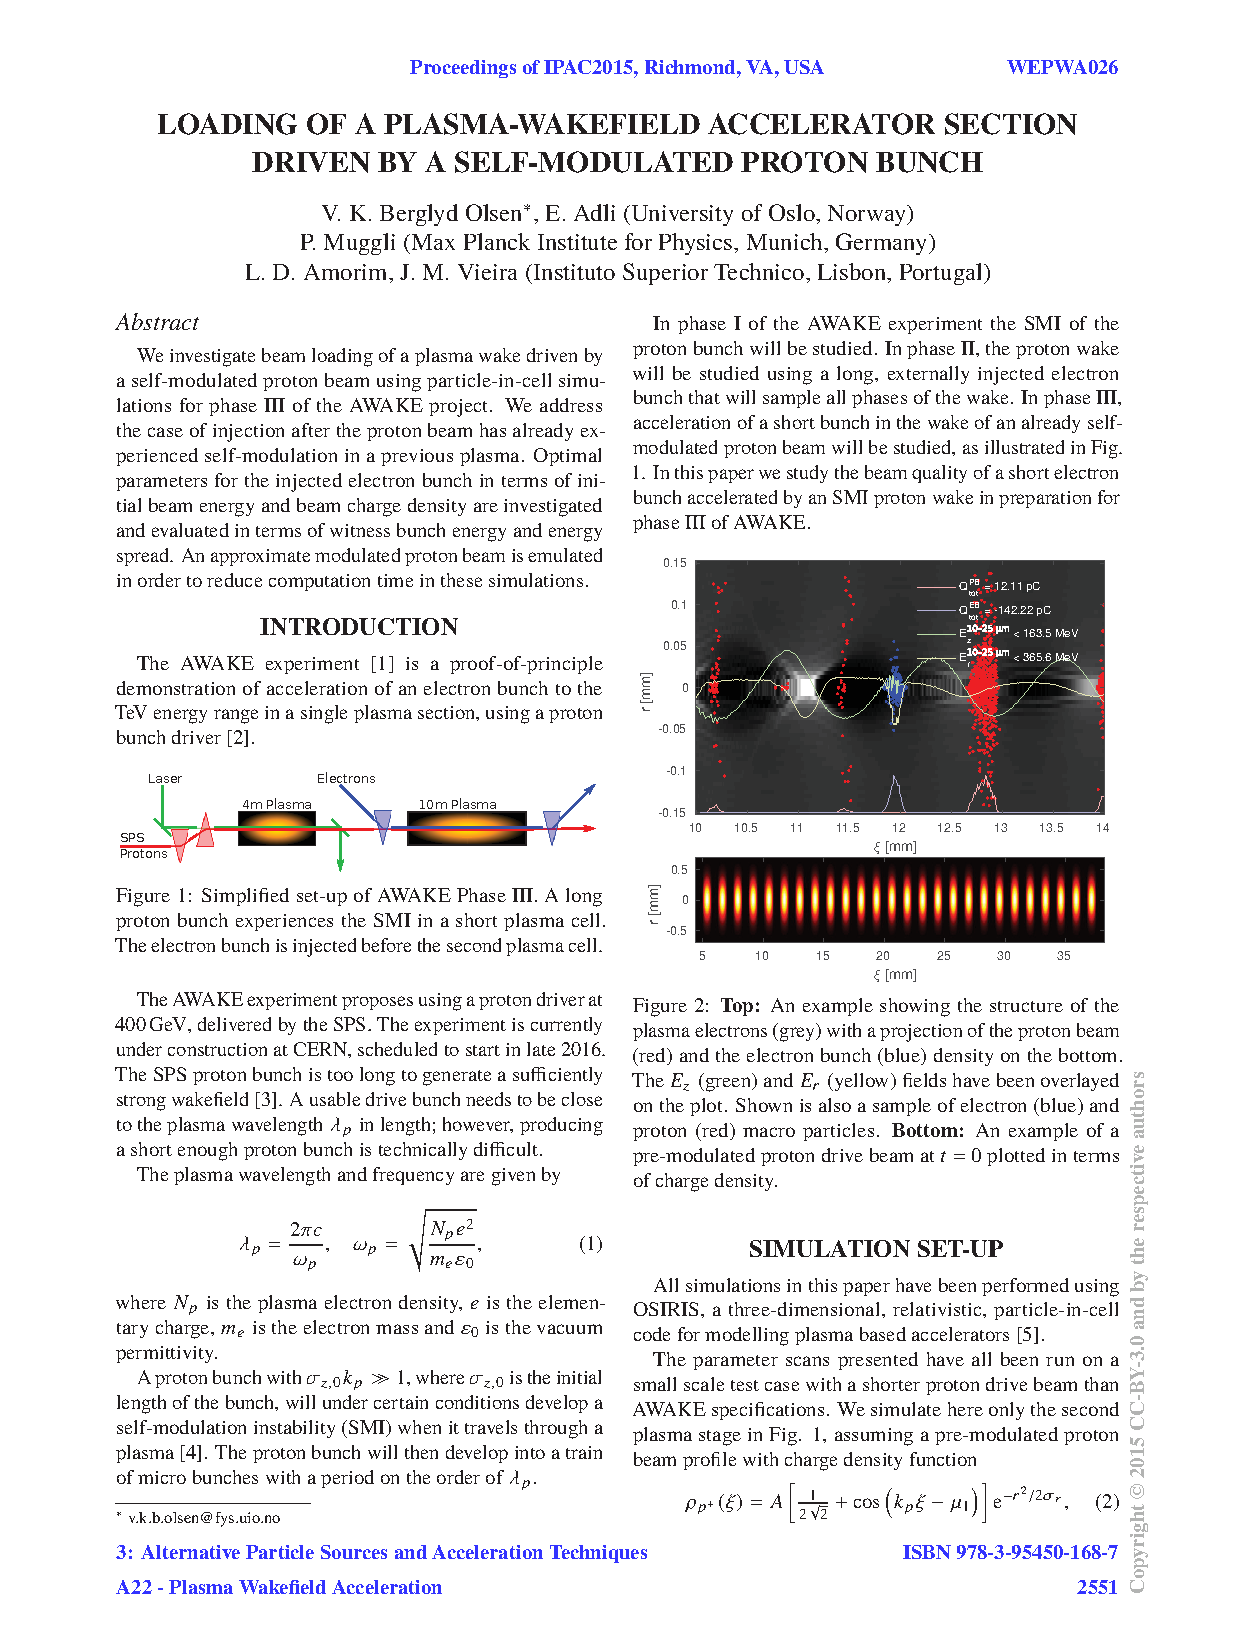
\includepdf[pages=1-last,openright,scale=0.95,pagecommand={}]{files/IPAC15-WEPWA026.pdf}
    %
%  Publication 2 :: NAPAC 2016
% =============================
%

\chapter{Loading of Wakefields in a Plasma Accelerator Section\\
         Driven by a Self-Modulated Proton Beam}
\label{Pub:NAPAC16}

\begin{hangparas}{10mm}{1}

    \textbf{Abstract:}
    Using parameters from the AWAKE project and particle-in-cell simulations we investigate beam loading of a plasma wake driven by a self-modulated proton beam. Addressing the case of injection of an electron witness bunch after the drive beam has already experienced self-modulation in a previous plasma, we optimise witness bunch parameters of size, charge and injection phase to maximise energy gain and minimise relative energy spread and emittance of the accelerated bunch.

    \vspace{5mm}

    \textbf{Authors:}
    Veronica K. Berglyd Olsen, Erik Adli (University of Oslo, Oslo, Norway)
    Patric Muggli (Max Planck Institute for Physics, Munich, Germany and CERN, Geneva, Switzerland)
    Jorge M. Vieira (Instituto Superior Technico, Lisbon, Portugal)

    \vspace{5mm}

    \textbf{Publication:}
    Proceedings of NAPAC 2016, Chicago, Illinois, USA

    \vspace{5mm}

    \textbf{Date:} 9\ts{th} to 14\ts{th} of October, 2016


\end{hangparas}

    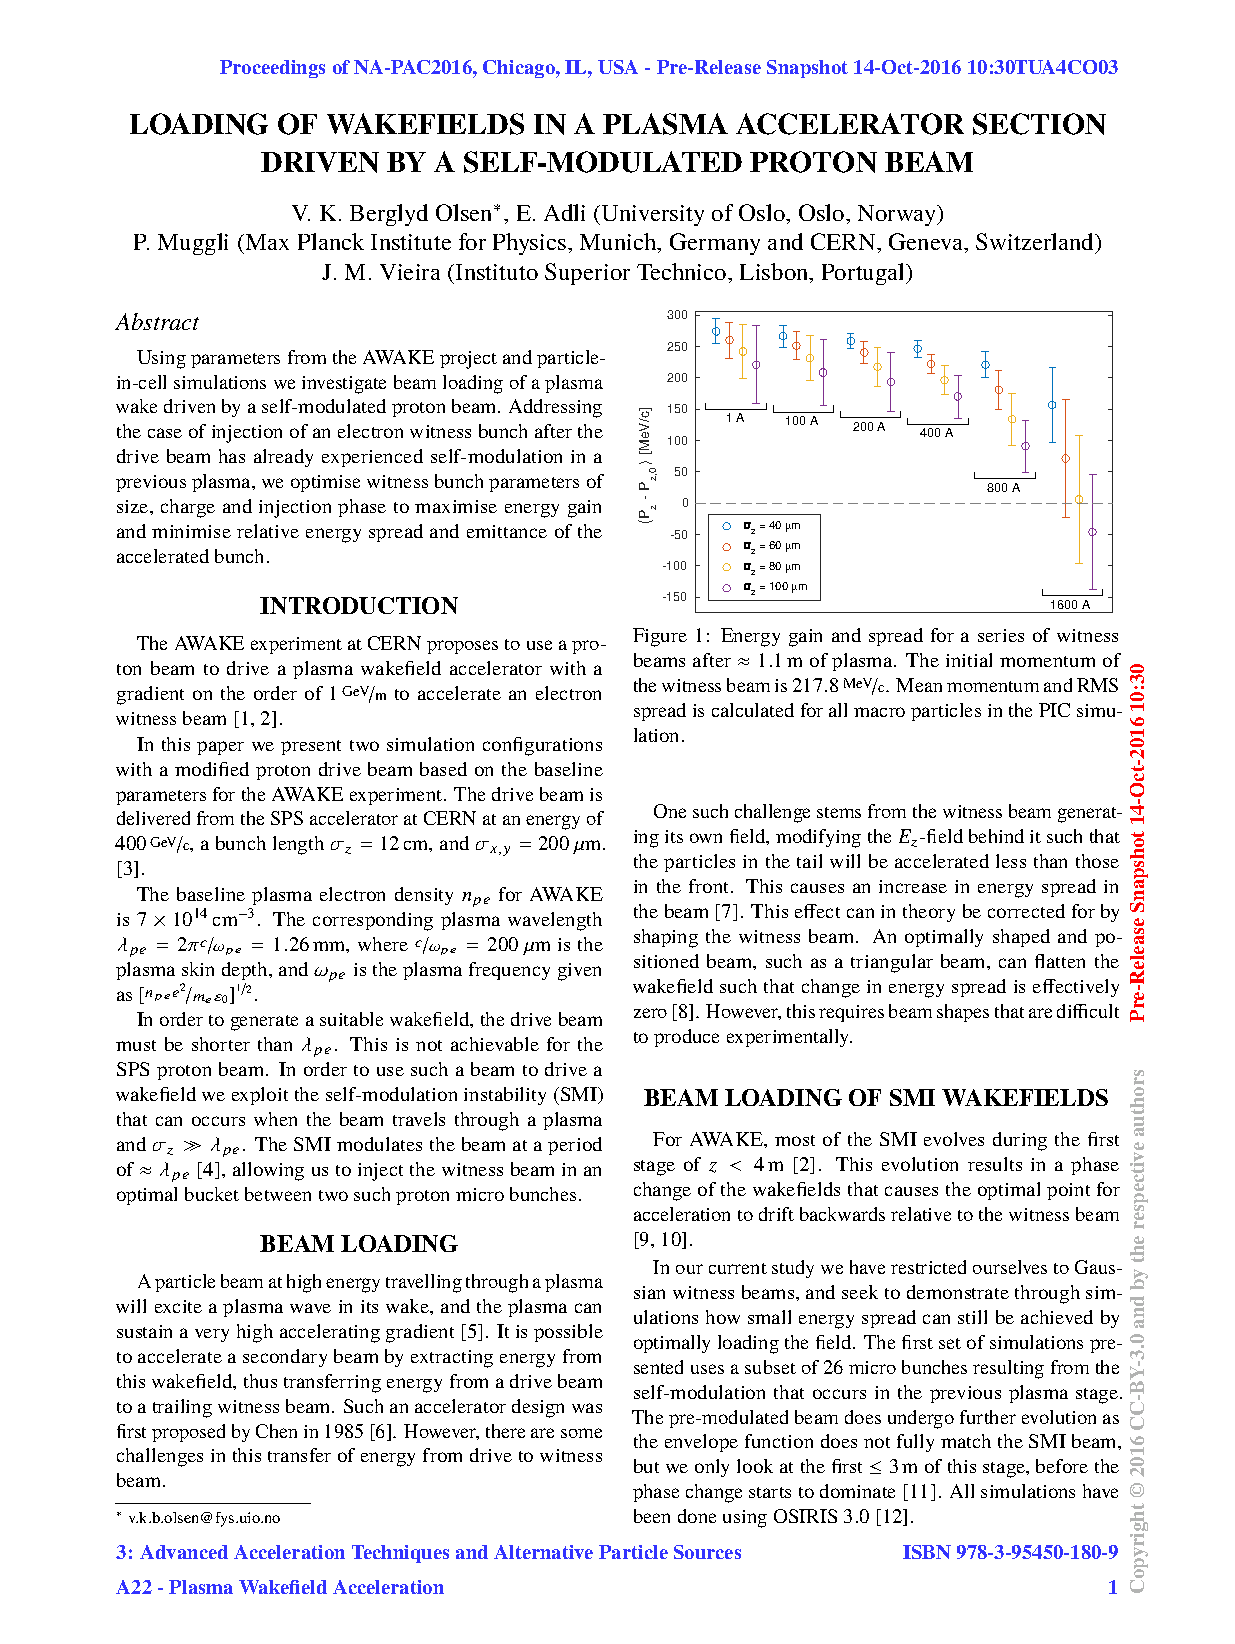
\includepdf[pages=1-last,openright,scale=0.95,pagecommand={}]{files/NAPAC16-TUA4CO03.pdf}
    %
%  Publication 4 :: IPAC 2017
% ============================
%

\chapter{Data Acquisition and Controls Integration of the AWAKE Experiment at CERN}
\label{Pub:IPAC17}

\begin{hangparas}{10mm}{1}

    \textbf{Abstract:}
    The AWAKE experiment has been successfully installed in the CNGS facility at CERN, and is     currently in its first stage of operation. The experiment seeks to demonstrate self-modulation of an SPS proton beam in a rubidium plasma, driving a wakefield of several gigavolt per meter. We describe the data acquisition and controls system of the AWAKE experiment, its integration into the CERN controls system and new control developments specifically required for the AWAKE experiment.

    \vspace{8mm}

    \textbf{Authors:}
    Veronica K. Berglyd Olsen (University of Oslo, Oslo),
    Spencer J. Gessner,
    Jozef J. Batkiewicz,
    Stephane Deghaye,
    Edda Gschwendtner (CERN, Geneva, Switzerland),
    Patric Muggli (Max Planck Institute for Physics, Munich, Germany and CERN, Geneva, Switzerland)

    \vspace{5mm}

    \textbf{Publication:}
    Proceedings of IPAC 2017, Copenhagen, Denmark

    \vspace{5mm}

    \textbf{Date:} 14\ts{th} to 19\ts{th} of May, 2017

\end{hangparas}

    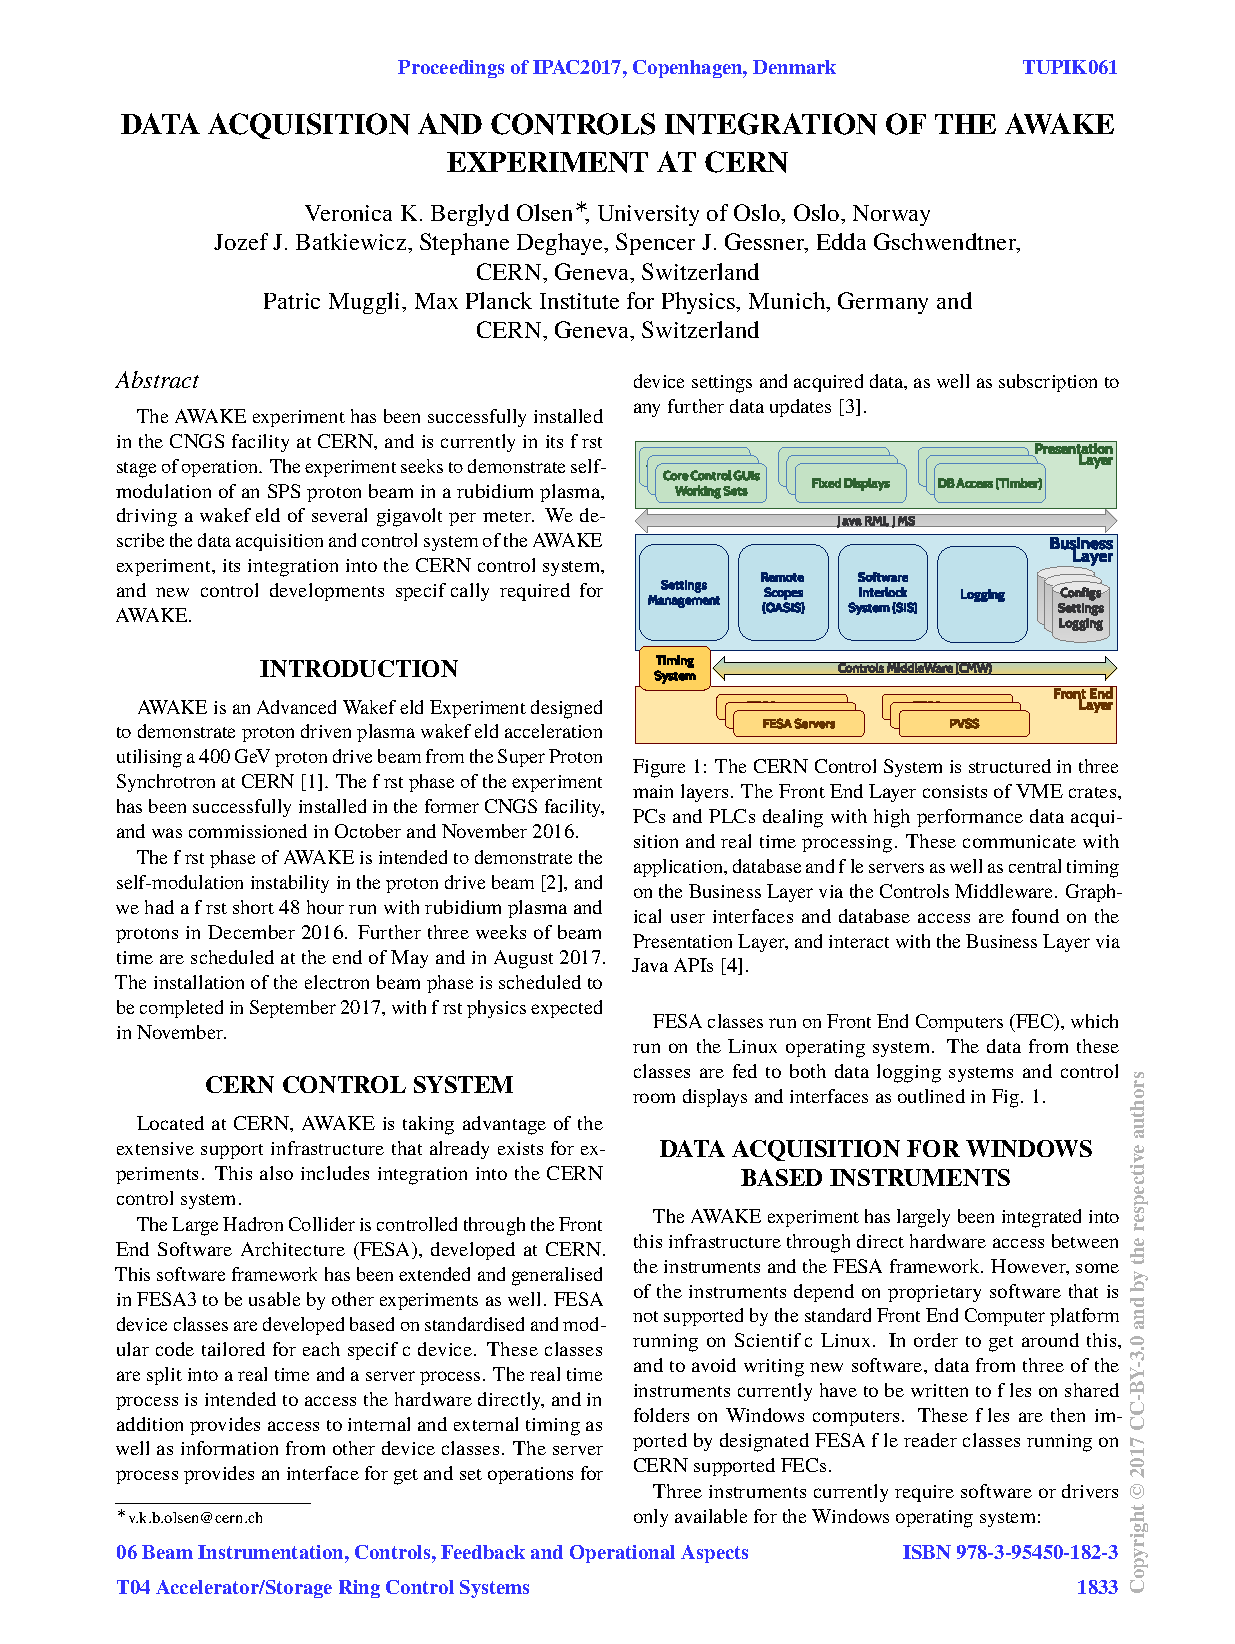
\includepdf[pages=1-last,openright,scale=0.95,pagecommand={}]{files/IPAC17-TUPIK061.pdf}
    %
%  Publication 3 :: Peer Review
% ==============================
%

\chapter{Placeholder Title}
\label{Pub:PRev17}

\begin{hangparas}{10mm}{1}

    \textbf{Abstract:}
    Abstract

    \vspace{8mm}

    \textbf{Authors:}
    Veronica K. Berglyd Olsen (University of Oslo, Oslo)

    \vspace{5mm}

    \textbf{Publication:}
    Journal

    \vspace{5mm}

    \textbf{Date:}

\end{hangparas}

    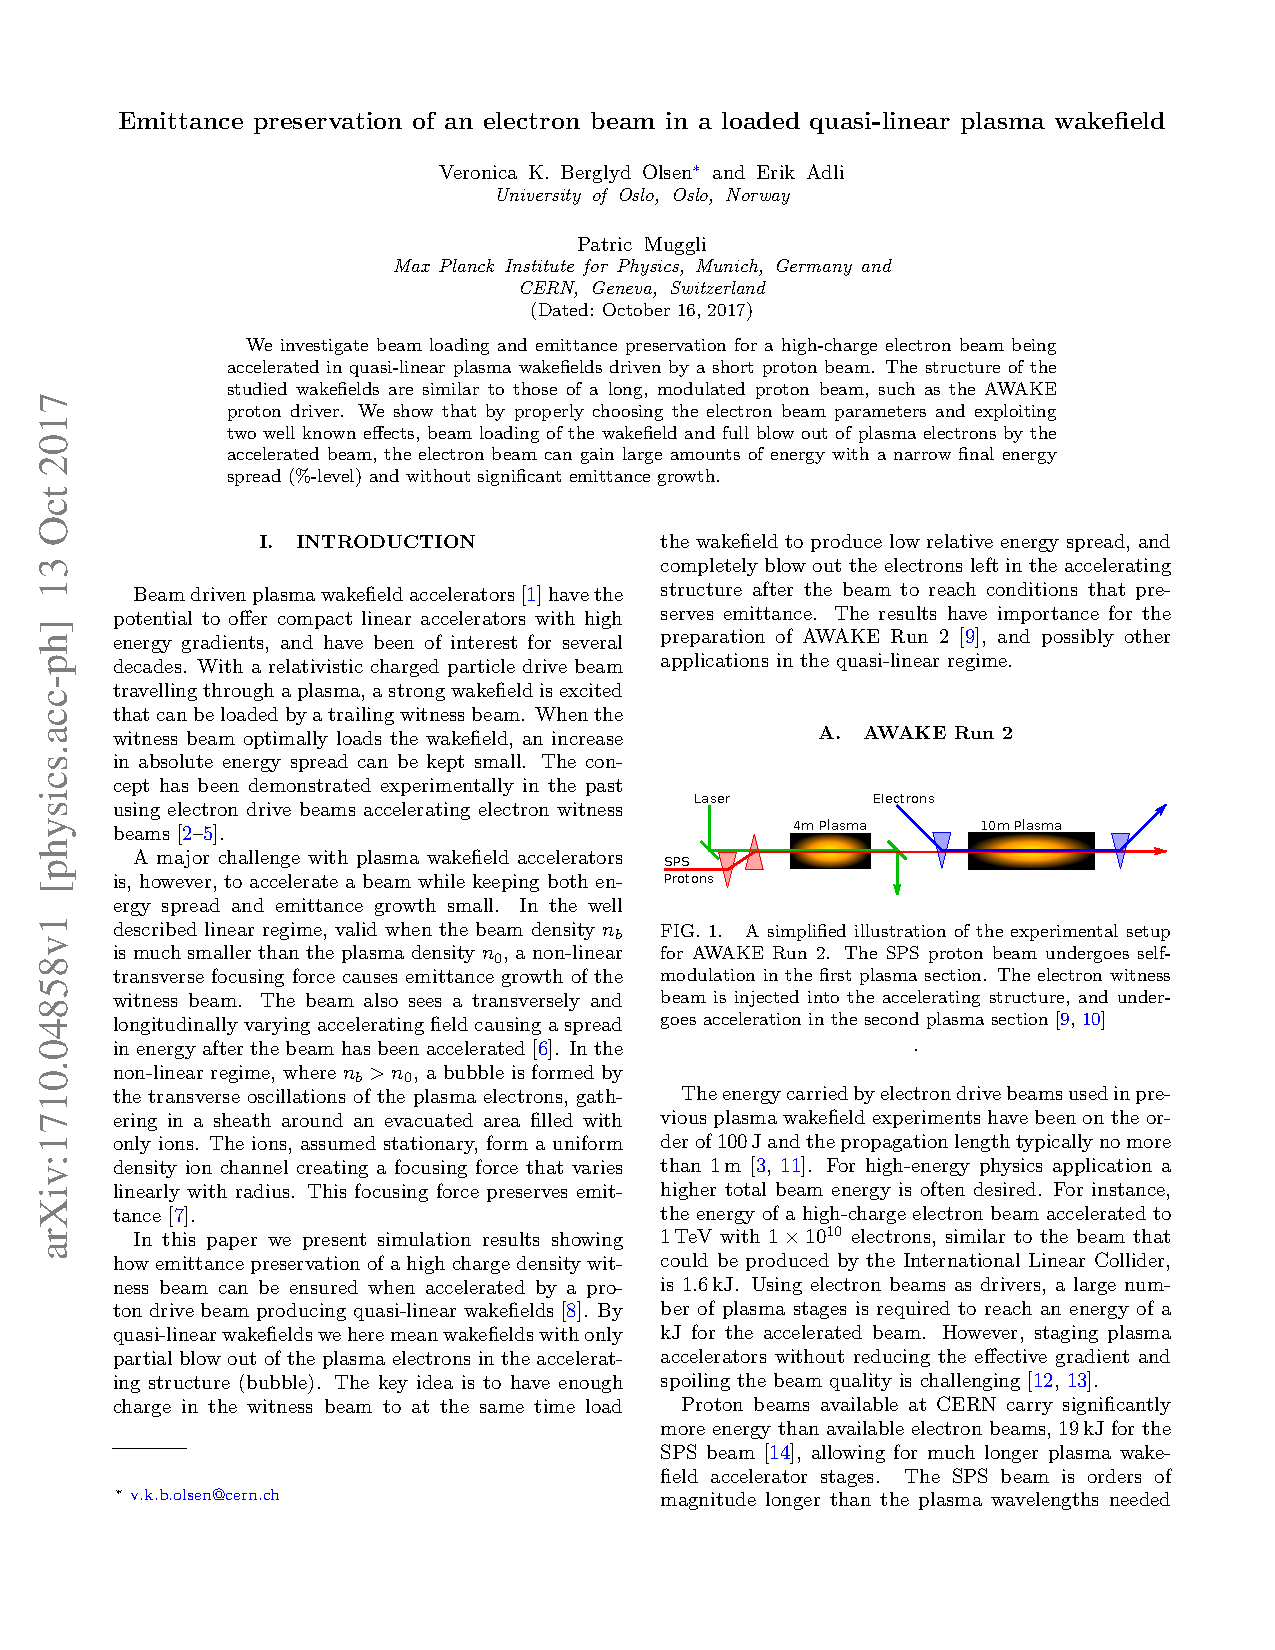
\includepdf[pages=1-last,openright,scale=0.95,pagecommand={}]{files/BeamLoading17.pdf}

% Appendices

\cleardoublepage
\bookmarksetup{startatroot}
\phantomsection
\part*{Appendices}
\label{A:App}

\renewcommand\appendixtocname{Appendices}
\renewcommand\appendixname{Appendix}

\appendix
    \setcounter{chapter}{0}
    \renewcommand{\thechapter}{\Alph{chapter}}
    \renewcommand{\theHchapter}{\Alph{chapter}}
    %
%  Appendix : PIC
% ================
%

\chapter{Particle in Cell (PIC)}
\label{Apx:PIC}

Some stuff about PIC codes

% ==================================================================================================================== %
\section{Numerical Cherencov}
\label{PIC:NumCher}

    %
%  Appendix : PIC
% ================
%

\chapter{Data Analysis}
\label{Apx:DA}

The OSIRIS simulation code does not include a data analysis framework. It has been very useful to develop a tool for effective analysis of the large amount of data produced by these simulations.

For the experiment itself a portion of the PhD project has been spent developing data acquistion tools and integrating these with the existing CERN data acquisition infrastructure.

As of the time of writing, the OsirisAnalysis framework is publicly available on GitHub \cite{berglyd_olsen_osirisanalysis:_2013}.

% =============================================================================================== %
\section{Osiris Analysis Framework}
\label{Tools:OA}

The OsirisAnalysis framweork is a modular and object oriented data analysis framweork written in MATLAB. It was designed as a three layer tool to wrap a single data set of OSIRIS simulation data.

\begin{itemize}
    \item \textbf{Layer 1:} Cosnists of the core datawrapper, OsirisData, which provides an interface through which raw data files as well as the simulation input file is parsed. It provides a uniform method for extracting data, and gives access to all the simulation parameters and conversion factors for converting Osiris' normalised units into SI units.
    \item \textbf{Layer 2:} The second layer consists of a set of classes that takes an OsirisData object as input, and returns standardised structs of data that can be scaled and converted to prefered units. They perform often needed tools and methods to parse data and extract more detailed information from the larger raw datasets.
    \item \textbf{Layer 3:} The third layer consist of a number of useful standardised plots and a GUI tool to quickly do a preliminary analysis of simulation data.
\end{itemize}

The philosophy behind this layering of the analysis tool is to allow the user the freedom to choose how many of these they will use. Only using the first layer will give the user access to all the simulation parameters as well as a method to extract data in a standardised manner and return a simple matrix of its content. Adding the second layer gives additional access to automatic unit conversion and other tools if needed. The third layer is entirely optional and simply provides a quick way to browse through the data.

% =============================================================================================== %
\subsection{OsirisAnalysis Core Objects}
\label{Tools:OALay1}

The innermost layer consists of two classes OsirisData and OsirisConfig.

The OsirisData class wraps the simulation data folder and is the core interface through which data is extracted. The class also provides some simple methods for extracting information about the dataset like physical dimensions of the beam and the distribution of the plasma.

The OsirisConfig class is a wrapper for the input file itself, and contains a parser for this file which extracts all the relevant information for both analysis and provides lists of available diagnostics for the graphical user interface (GUI). All conversion factors to SI units are calculated on the fly when the input file is loaded. The OsirisConfig class is not intended to be called by the user, but is found as a child object of the OsirisData data object.

% =============================================================================================== %
\subsection{OsirisAnalysis Data Types}
\label{Tools:OALay2}

The secondary layer of the OsirisAnalysis framework is a set of subclasses under a parent class named OsirisType. The subclasses will give access to specific types of data more or less directly related to the diagnostics types produced by the OSIRIS simulation code.

The classes provided are:

\begin{itemize}
    \item \textbf{Density and Field:} These are classes that produce grid diagnostics data for the particle density data dumps or the field diagnostics data. They support all the different density diagnostics outputs of Osiris, and will in addition calculate the wakefields from the magnetic and electric fields given by $W = F/q = E - v \times B$.
    \item \textbf{Momentum:} The Momentum class consists of a set of methods that will calculate the evolution of the beams energy and momentum over several time dumps.
    \item \textbf{Phase:} The Phase class provides several tools for phase space diagnostics, including calculations of Twiss parameters.
    \item \textbf{UDist:} This class is similar to the Dnesity and Field classes, and provides methods to process velocity and thermal distribution data.
    \item \textbf{Species:} The Species class provides a few additional specialised tools for calculating energy deposition and gain into and from the plasma by the beams, and is also the class where particle tracking data is parsed.
\end{itemize}

In addition to these data parsing classes, there is also a Variables class that will translate Osiris diagnostics variables into readable forms and into strings usable for plot labels. There is also a MathFunc class that provides a math parser that emulates the one used by OSIRIS to parse mathematical functions from the input files. This class is mainly used to extract geometric information about beam density based on the function provided in the input file without the need to first run the code to provide raw particle data.

% =============================================================================================== %
\subsection{OsirisAnalysis Graphical Interface and Plots}
\label{Tools:OALay3}

The final layer of the OsirisAnalysis framwork is a set of very flexible plotting tools. Most of them have a long list of optional input argument. Most of these optional arguments are available through a graphical interface also written in MATLAB named AnalysisGUI.


% Back Matters

\backmatter
\bookmarksetup{startatroot}
\cleardoublepage
\phantomsection
\addcontentsline{toc}{chapter}{Bibliography}
\bibliography{Bibliography,Additional}
\null

\phantomsection
\bookmarksetup{startatroot}
\pdfbookmark{End}{EndOfDoc}
\vspace*{\fill}
\footnotesize
\noindent Document compiled on \today~at~\currenttime
\newline
\pdftexbanner

\end{document}

% ================================================================================================ %
